%&"../net"
% Reference:
% https://shimowendang.com/docs/wGQPHvHrcTTDyChh/read
\endofdump
\tikzexternalize[prefix=cache/]{lab03}
\begin{document}
\title{Socket Programming}
\maketitle
\tableofcontents

\vfill
You will implement a simple file share application using TCP Socket APIs. 

You can use any programming language. You need to submit your code together with a report. The report should contain how to run your program and some evaluation results.
\vfill
\clearpage
\section{C/S 模型}

\subsection{C/S 模型要求}

\begin{enumerate}
    \item Implement C/S model: 
    \begin{enumerate}
        \item Server listens to a given port (>1024, e.g. 2680)
        \item Multiple clients request the same file from the server
        \item Each client save the file to its local directory.
    \end{enumerate}
    \item Use Mininet to compare the overall file downloading time. Study how the number of downloading time changes with respect to the number of peers. You need to create the following star topology in Mininet. You can use one host as a server, and the other hosts as peers requesting files.
    \begin{figure}[H]
        \centering
        \begin{tikzpicture}[font=\Large]
\node (s) at (0,0) {\faServer};
\node (c1) at (0,2) {\faLaptop};
\node (c2) at (2,1) {\faLaptop};
\node (c3) at (2,-1) {\faLaptop};
\node (c4) at (0,-2) {\faLaptop};
\node (c5) at (-2,-1) {\faLaptop};
\node (c6) at (-2,1) {\faLaptop};
\draw  (c1) edge (s);
\draw  (c2) edge (s);
\draw  (c3) edge (s);
\draw  (c4) edge (s);
\draw  (c5) edge (s);
\draw  (c6) edge (s);
\end{tikzpicture}
    \end{figure}
\end{enumerate}

\subsection{C/S 模型测试}

\subsubsection{批量测试}

\begin{lstlisting}[style=commandshell]
cd csmodel
./cstest.sh
\end{lstlisting}

这将会生成 10 MB 的随机文件 \verb"file.txt",运行 Python \faPython\ 版本的脚本进行模拟。

由图 \ref{fig:csmodelstat} 可见,随着客户机的增长,传输时间也会线性变长。

\begin{figure}[H]
    \centering
    \begin{tikzpicture}
        \begin{axis}[xmin={0},
        ymin={0},
        xlabel={\# Client},
        ylabel={Avg Transfer Time (s)},
        grid={major},
        ]
         \addplot+ [] table[] {csmodel/avgres_py.dat};
        \end{axis}
    \end{tikzpicture}
    \caption{不同的客户机数量下平均传输时间}\label{fig:csmodelstat}
\end{figure}    

\code[language=bash]{csmodel/cstest.sh}

% 如果遇到意外中断,可以使用 mn 命令清除所有连接。

\subsubsection{单次测试}

\begin{lstlisting}[style=commandshell]
python centralized.py [hostnumber] [py|c] [--dirty]

# [hostnumber] is the number of hosts in the structure (including the server)
# py will launch python script, while c will launch c version.
# --dirty will pass all the checking
\end{lstlisting}

使用 \verb"python" 运行 \verb"csmodel/centralized.py" 脚本即可开始测试星状结构的网络。如果没有给定主机数量,运行脚本后就会提示输入。如果脚本后面添加参数 \verb" py --dirty" 则可以跳过一些检查,这对于客户机数量多的情况比较有用。

\begin{figure}[H]
    \centering
    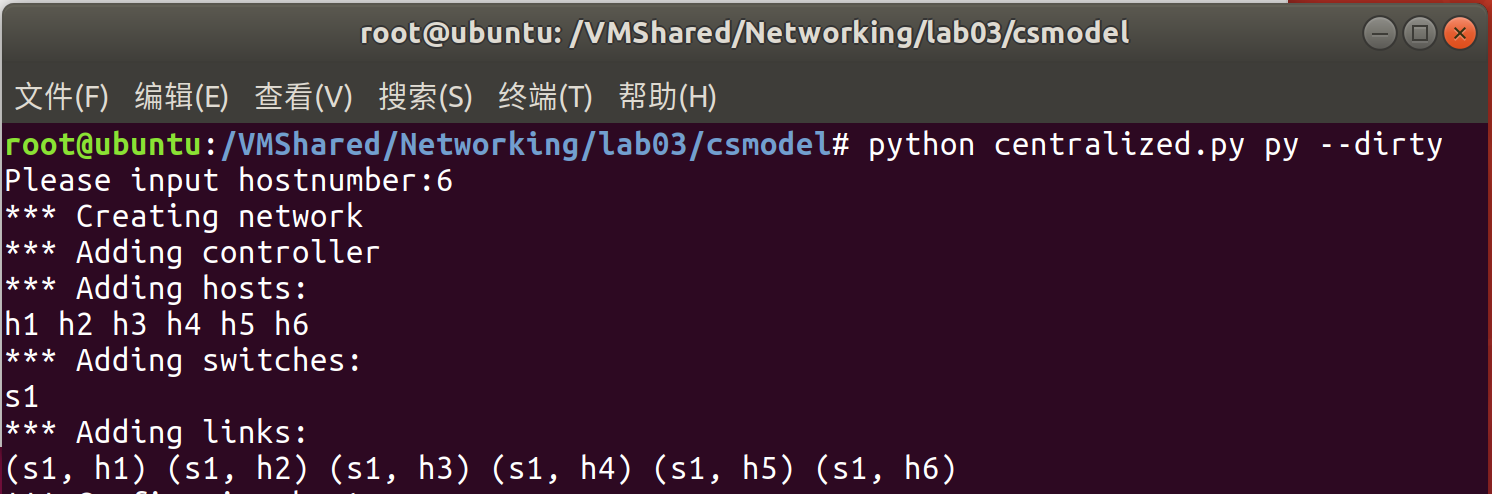
\includegraphics[width=\linewidth]{runcsmodel}
    \caption{C/S Mininet 测试}\label{fig:csmodelrun}
\end{figure}

C/S 模型架构实现代码见附录 \ref{sec:cscentralized}。由图 \ref{fig:csmodeltest} 所示,所有的客户机会\emph{同时}从服务器获取上述的 10 MB 文件,每个客户机会在完成传输后各自存储为对应的 \verb"file_receive_h*.txt" 文件,并将计时结果写入文件 \verb"result_py.dat"。由于最后一个主机进程会阻塞 Mininet 测试主线程,所以最后一个结束后,等待片刻,就会对结果进行统计,并给出平均时间。

\begin{figure}[H]
    \centering
    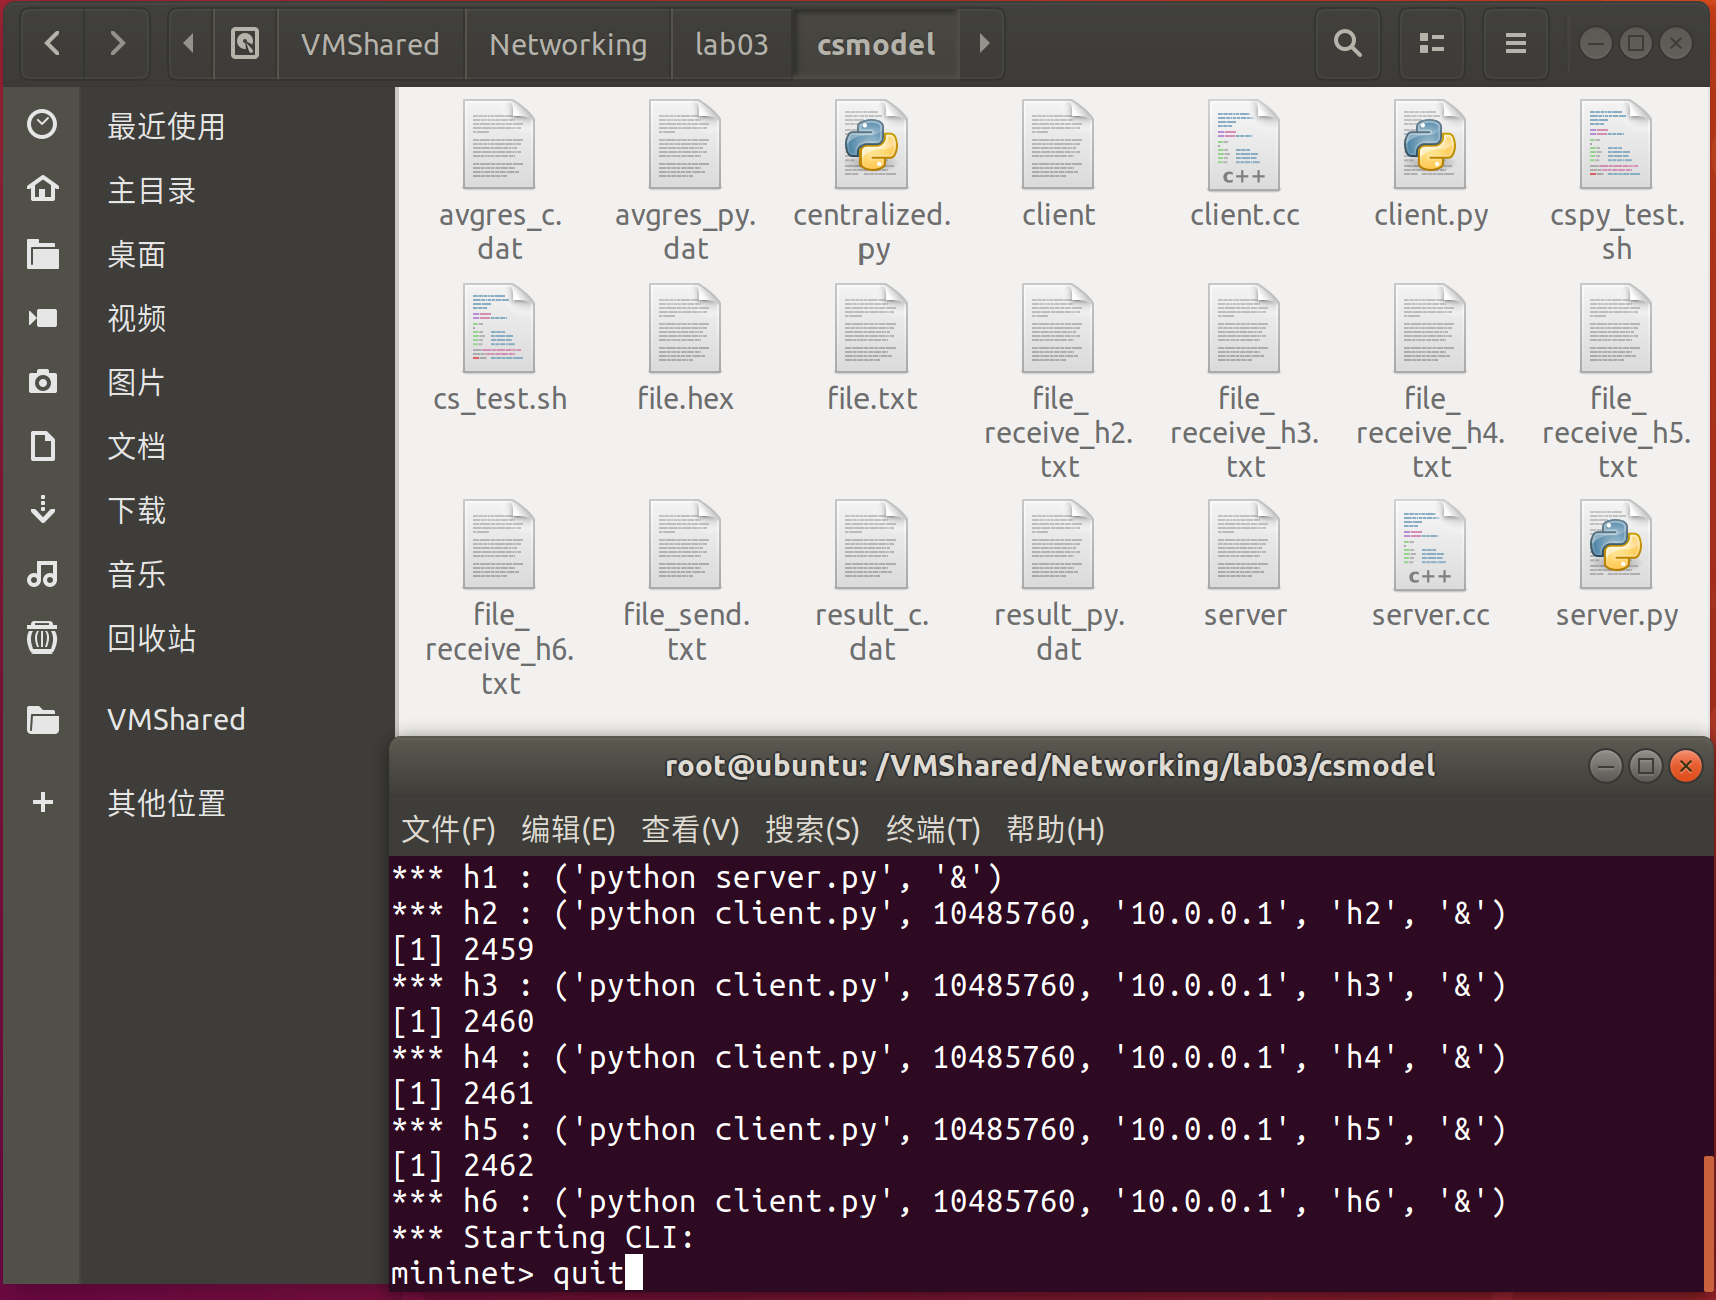
\includegraphics[width=0.5\linewidth]{centralized}
    \caption{运行多机测试}\label{fig:csmodeltest}
\end{figure}

\subsubsection{单机测试}

\begin{lstlisting}[style=commandshell]
./cspy_test.sh
\end{lstlisting}
 
使用 \verb"csmodel" 文件夹下的 \verb"cspy_test.sh" 脚本即可测试 Python \faPython\ 版本的单服务器---单客户端模型,在 \verb"2683" 端口上传输 10 MB 的文件,传输时长大概在 4s 左右。如果最后没有比较上的异常,就说明被完整地传输了。

\begin{figure}[H]
    \centering
    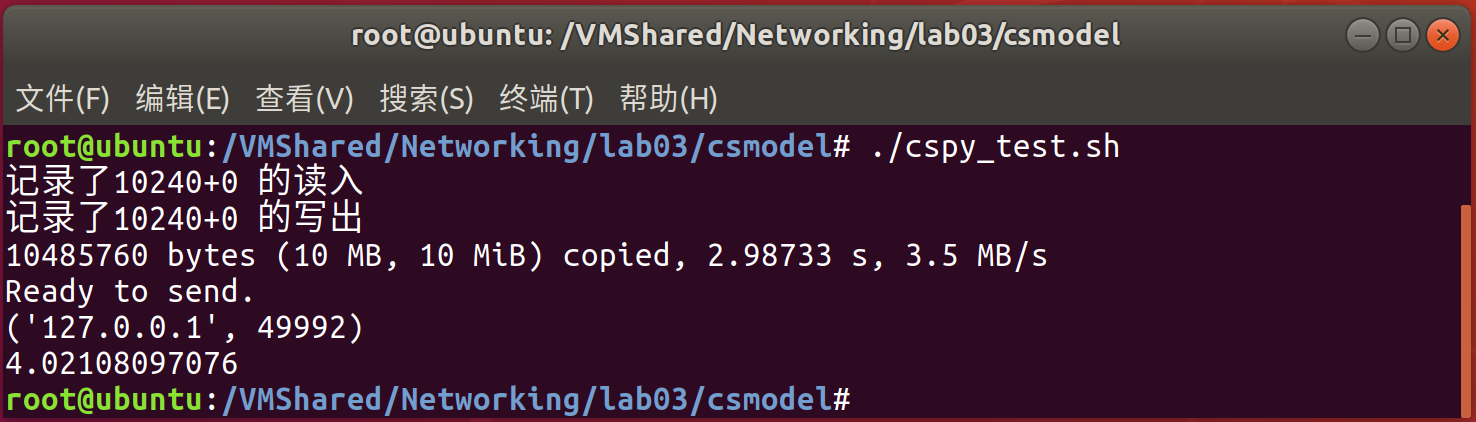
\includegraphics[width=\linewidth]{cspytest}
    \caption{单机测试}
\end{figure}

\code[language=bash]{csmodel/cspy\_test.sh}

C/S 模型的服务器和客户端 Python \faPython\ 实现见附录 \ref{sec:cspython}。

当然也参考着示例代码实现了 C 语言版本,详见附录 \ref{sec:csc}。C 语言实现版本的速度快很多,基本上不会超过 0.5s 就可以完成上面 Python 的操作,这样会导致数据差别小,就不给出 C 语言测试版本的运行时间测试了,注意 C 语言版本使用了 2680 端口。

\section{P2P 模型}

\subsection{P2P 模型要求}

\begin{enumerate}
    \item Implement P2P model: Each peer downloads part of the file from the server, and then distributes it to all the other peers.

    \item Use Mininet to compare the overall file downloading time under P2P model.
    
    \item For peer-to-peer mode, you may want to design a tracker file first. The tracker file contains the following information:
    
    \begin{table}[H]
    \centering
    \begin{tabular}{ll}
        \toprule
        file chunk id & peer ip \\
        \midrule
        1 & 10.0.0.1\\
        2 & 10.0.0.2\\
        3 & 10.0.0.3\\
        4 & 10.0.0.4\\
        \bottomrule
    \end{tabular}
    \end{table}

    Then, if a client wants piece 2, it will contact 10.0.0.2. If the peer with ip=10.0.0.2 does not have the piece yet, it will contact the server to download this piece first. 
\end{enumerate}

\subsection{P2P 模型测试}

\subsubsection{批量测试}

\begin{lstlisting}[style=commandshell]
cd p2pmodel
./p2ptest.sh
\end{lstlisting}

使用 \verb"p2pmodel/p2ptest.sh" 可以进行批量测试,这一步可以创建一个 10MB 大小的文件 \verb"file.txt"。图 \ref{fig:p2pmodelstat} 显示了对等方的数目多少不会导致传输时间的太大波动,至少不是 C/S 模型的线性增长。

\begin{figure}[H]
    \centering
    \begin{tikzpicture}
        \begin{axis}[xmin={0},
        ymin={0},
        xlabel={\# Peer},
        ylabel={Avg Transfer Time (s)},
        grid={major},
        ]
        \pgfplotsset{cycle list shift=1};
         \addplot+ [] table[] {p2pmodel/avgres_py.dat};
        \end{axis}
    \end{tikzpicture}
    \caption{不同的对等方数量下平均传输时间}\label{fig:p2pmodelstat}
\end{figure}

\code[language=bash]{p2pmodel/p2ptest.sh}

\subsubsection{单次测试}

当然也可以直接运行 \verb"python" 脚本进行测试:
\begin{lstlisting}[style=commandshell]
python centralized.py 5
\end{lstlisting}
最后一个参数用于指定主机数量。请注意,应当先生成文件再进行单次测试。

\begin{figure}[H]
    \centering
    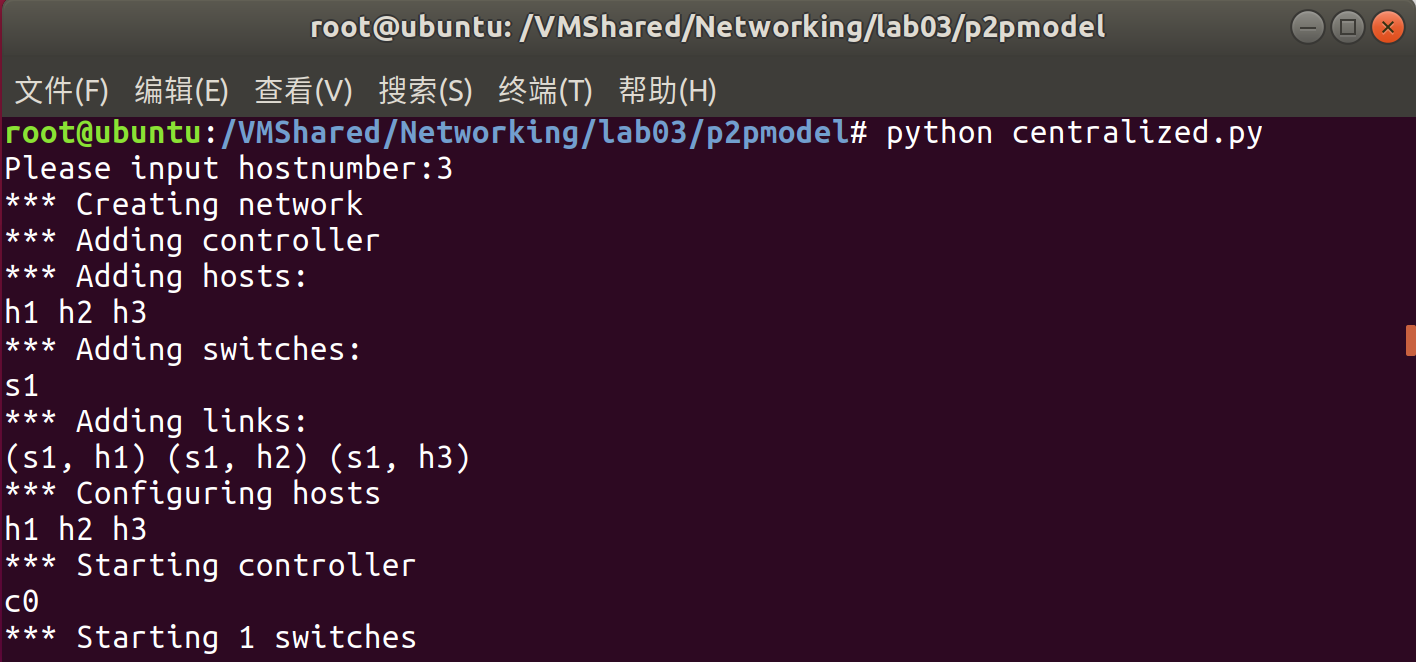
\includegraphics[width=\linewidth]{runp2pmodel}
    \caption{P2P Mininet 测试}\label{fig:p2pmodelrun}
\end{figure}

附录 \ref{sec:p2pcentralized} 显示了 P2P 模型的 Mininet 架构实现。制定了主机数量后,会生成对应的 \verb"tracker.dat" 文件,和题设一样的格式。

附录 \ref{sec:p2ppy} 显示了 P2P 模型的服务端和对等端实现。关于对等方,重要的一点是每个对等方也会新建一个服务器线程,以向其他对等方发送数据,如果本地没有文件,就会先阻塞地向服务器获取数据。对等端内部会使用一个数据结构存储已经得到的文件块信息,最后会等待所有向其他对等方的传输线程终止,才会准备将数据写入文件。由于实现起来较为复杂,就不提供 C 语言实现版本。

\section{结论}

\begin{figure}[H]
    \centering
    \begin{tikzpicture}
        \begin{axis}[xmin={0},
        ymin={0},
        xlabel={\# Client / \# Peer},
        ylabel={Avg Transfer Time (s)},
        grid={major},
        ]
        \addplot+ [] table[] {csmodel/avgres_py.dat};
         \addplot+ [] table[] {p2pmodel/avgres_py.dat};
         \legend{C/S,P2P}
        \end{axis}
    \end{tikzpicture}
    \caption{平均传输时间比较 \faPython}\label{fig:p2pmodelstat}
\end{figure}

将统计数据放在一张图上,会发现后面 C/S 模型仍然在线性增长,而 P2P 模型并不怎么增长。而 P2P 在创建线程(增加连接数)上的开销要比 C/S 模型大很多,使用本地虚拟机的 Mininet 模拟会在这个方面遭受性能问题,对等方数目再多甚至会报错。

\appendix

\section{C/S 模型架构实现}\label{sec:cscentralized}

下面给出了 Mininet 配置的具体代码。实际上星状网络可以采用 \verb"LinearTopo" 代替,此处为了更好地控制源码,就采用了手写的 \verb"CentralizedTopo" 网络结构。\verb"dumpNodeConnection" 是重要的,这样才可以防止 IP 地址被重复使用。

\code{csmodel/centralized.py}

\section{C/S 模型 Python 实现 \faPython}\label{sec:cspython}

为了方便理解 TCP 网络模型,先跟着书用 Python 实现了一遍多线程 C/S 模型。

下面是服务器端的代码,在主循环中由 \verb"accept()" 阻塞接收,一旦有客户机进入就会开辟新的线程进行文件传输。

\code{csmodel/server.py}

下面是客户端代码,由于 TCP 连接接收大小有一定的限制,超过限制可能就会产生长期接收不到的情况,所以每次只会接收 1024 字节,分为多次进行接收。由于 Python 内存访问比较慢,这里直接就写入了文件,没有首先将内容进入内存。

\code{csmodel/client.py}

\section{C/S 模型 C 实现 \textsf{C}}\label{sec:csc}

如果想运行 C 语言版本,进行单机测试:
\begin{figure}[H]
    \centering
    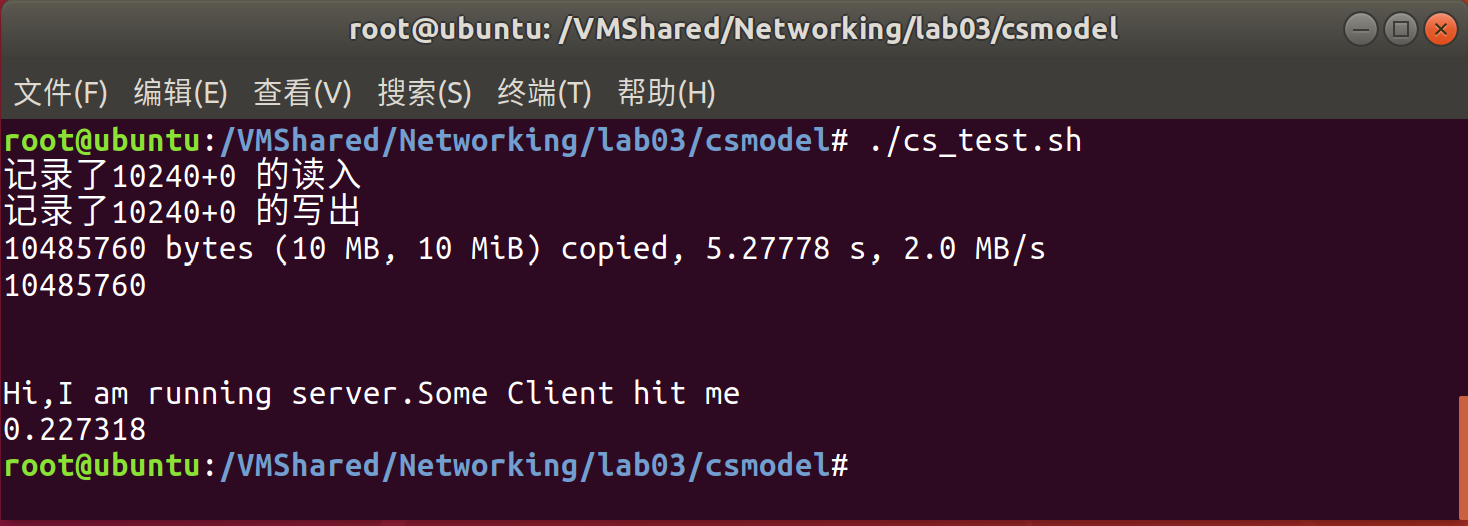
\includegraphics[width=0.7\textwidth]{cstest}
    \caption{C 语言单机测试}
\end{figure}

进行 Mininet 测试需要使用参数 \verb" c --dirty"。

\begin{figure}[H]
    \centering
    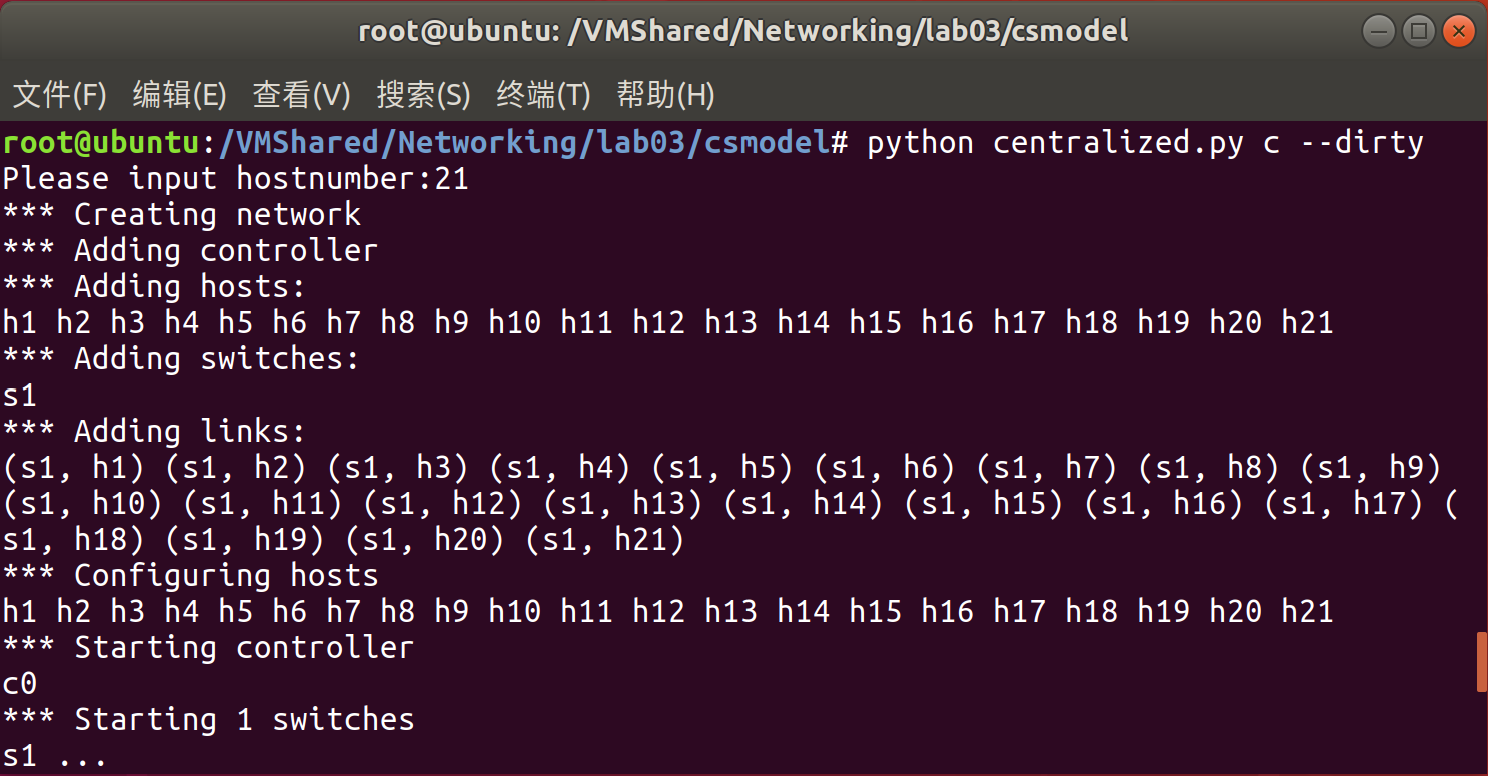
\includegraphics[width=0.6\textwidth]{cruncsmodel}
    \caption{C 语言多机测试}
\end{figure}

可见使用 C 语言效率更高,1s 不到就可以完成,这也导致如果需要对其评测需要使用很大的文件,否则数据差距并不明显,这里就跳过对 C 语言实现版本的测评部分。下面的代码主要是对示例代码的一些改进而得到的。

\code[language=c]{csmodel/server.cc}

服务器会首先读取文件数据。与一个客户机建立连接后,就会开辟一个新的线程,但是这个线程会与主线程显式脱离,以传输数据。

\code[language=c]{csmodel/client.cc}

客户端会首先将数据存储在内存中,再写入文件。

\section{P2P 模型架构实现}\label{sec:p2pcentralized}

\code{p2pmodel/centralized.py}

\section{P2P 模型 Python 实现 \faPython}\label{sec:p2ppy}

服务器与 C/S 模型的差距不大,主要可以接收一个文件块的参数。

\code{p2pmodel/server.py}

对等方的实现相对复杂。主要有两种线程:\verb"ServiceThread" 用于向其他对等方提供服务(或者会向服务器获取数据,如果最后没有完整传输,会强制从服务器获取对应的数据);另一方面,\verb"FetchingThread" 用于从其他对等方获取数据,并在最后合并到主线程。

由于数据上并没有线程间依赖,所以可以不加线程锁进行同步,编程上在这方面也有着对应的考虑。有时候对等方的服务线程可能还没有开启,会有失联的情况,这时会尝试一次重连,基本上都可以正确传输(对等方数目适当的情况下)。

\code{p2pmodel/peer.py}

\end{document}